\begin{frame}[label=Funzione]
  \frametitle{Funzione}
  \begin{block}{Funzione}    
  La nozione di \textit{funzione} viene introdotta e precisata in molti modi diversi
  durante il XVII secolo.

  Nella cinematica si hanno quantità variabili con il tempo, ovvero funzioni del tempo. 
  Si arriva in questo modo alle \textit{fluenti} di Newton.

  Per contro Descartes aveva escluso dalla ``geometria'' tutte le curve non analitiche (trascendenti o meccaniche).
  Inoltre il successo degli sviluppi in serie di Newton, creò confusione fra funzioni
  suscettibili di definizione analitica e funzioni sviluppabili come serie di potenze (p.e.$sen(x)$).  
  
  Leibniz introduce i termini "costante","variabile" e "parametro".
  Nella sua corrispondenza con Bernoulli, propone $x\bigsqcup$ ove noi scriviamo $f(x)$ notazione introdotta da Eulero.
  
  Cauchy definisce la funzione come facciamo noi oggi. Da essa derivano facilmente le nozioni di limite e di derivata la cui
  esistenza cessa di essere un articolo di fede, ma un problema da studiare con
  gli strumenti dell'analisi.
  Per l'integrale definito, Cauchy fa adottare la notazione $\int_{a}^bf(x)dx$ proposta da Fourier
  al posto della scomoda $\int f(x)dx$ $\left[\begin{array}{c} x=a \\ x=b \end{array}\right] $ di Eulero
  \end{block}  
\end{frame}

\begin{frame}[label=Cauchy]
  \frametitle{Cauchy}

  \begin{block}{Prima definizione di integrale.} 
    Nel 1821, A.L.Cauchy diede la prima definzione precisa di integrale 
    $\int_{a}^bf(x)dx$. Egli divise l'intervallo di estremi $a$ e $b$ 
    in un numero finito di sottointervalli aventi estremi.
    \begin{center}
      $a = x_0 < x_1 < ... < x_{n-1} < x_n = b$
    \end{center} 
    per poi considerare la somma finita
    \begin{center}
      $(x_1 - x_0)f(x_0) + (x_2-x_1)f(x_1) + ... + (x_n - x_{n-1})f(x_{n-1}) $
    \end{center}
    che rappresenta l'area totale dei rettangoli in figura.\\
    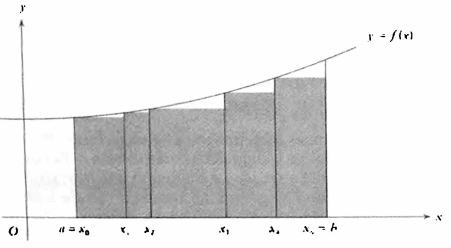
\includegraphics[width=0.5\textwidth]{Area-Cauchy.png}
  \end{block}
\end{frame}

\begin{frame}
  \begin{block}{Integrale come limite.}

    \alert{Ammesso che la cosa sia possibile}, l'area sottesa alla curva,
    è il numero approssimato da somme di questo genere, quando l'ampiezza dei rettangoli
    tende a zero. 
    Cauchy definí l'integrale $\int_{a}^bf(x)dx$ come il valore limite, quando esiste,
    di queste somme.
    Dimostrò inoltre che l'esistenza dell'integrale dipende dall'essere al curva $y=f(x)$ \textit{continua},
    dopo aver definito il concetto di \textit{continuità}.


  \begin{enumerate}
    \item Sia $f: [a,b] \rightarrow \mathbb{R}$ una funzione \textit{continua}
    \item Dividiamo $[a,b]$ in N parti uguali medianti i punti $x_i := a + i\frac{b-a}{N}$ 
    \item Definiamo \scalebox{1.5}{%
    $\int_{a}^{b} f(x) \,dx := \lim_{N \to +\infty}\sum_{i=0}^{N} f(x_{i-1}) \frac{b-a}{N}$      
    }
  \end{enumerate}

  Data l'ipotesi di continuità il limite esiste.
  \end{block}

  \begin{block}{La continuità}
    Una funzione $f$ è \textit{continua in x} se la differenza $f(x+\alpha) - f(\alpha)$ 
    tende a zero quando $\alpha$ tende a zero> $f$ è \textit{continua} se lo è in ogni
    punto del dominio di definizione.
  \end{block}


\end{frame}


